%-----------------------------------
% Define document and include general packages
%-----------------------------------
% Tabellen- und Abbildungsverzeichnis stehen normalerweise nicht im
% Inhaltsverzeichnis. Gleiches gilt für das Abkürzungsverzeichnis (siehe unten).
% Manche Dozenten bemängeln das. Die Optionen 'listof=totoc,bibliography=totoc'
% geben das Tabellen- und Abbildungsverzeichnis im Inhaltsverzeichnis (toc=Table
% of Content) aus.
% Da es aber verschiedene Regelungen je nach Dozent geben kann, werden hier
% beide Varianten dargestellt.
\documentclass[12pt,oneside,titlepage,listof=totoc,bibliography=totoc]{scrartcl}
%\documentclass[12pt,oneside,titlepage]{scrartcl}

%-----------------------------------
% Dokumentensprache
%-----------------------------------
%\def\FOMEN{}% Auskommentieren um die Dokumentensprache auf englisch zu ändern
\newif\ifde
\newif\ifen

%-----------------------------------
% Meta informationen
%-----------------------------------
%-----------------------------------
% Meta Informationen zur Arbeit
%-----------------------------------

% Autor
\newcommand{\myAutor}{Alexander Langel}

% Adresse
\newcommand{\myAdresse}{Kendelweg 16, 47179 Duisburg}

% Titel der Arbeit
\newcommand{\myTitel}{Aufbau einer Datensammlungsumgebung für Nachrichtenartikel}

% Betreuer
\newcommand{\myBetreuer}{Prof. Dr. Michael Colombo}

% Lehrveranstaltung
\newcommand{\myLehrveranstaltung}{Analyse semi- \& unstrukturierter Daten}

% Matrikelnummer
\newcommand{\myMatrikelNr}{487382}

% Ort
\newcommand{\myOrt}{DLS Studium}

% Datum der Abgabe
\newcommand{\myAbgabeDatum}{\today}

% Semesterzahl
\newcommand{\mySemesterZahl}{2}

% Name der Hochschule
\newcommand{\myHochschulName}{FOM Hochschule für Oekonomie \& Management}

% Standort der Hochschule
\newcommand{\myHochschulStandort}{DLS Studium}

% Studiengang
\newcommand{\myStudiengang}{Big Data \& Business Analytics}

% Art der Arbeit
\newcommand{\myThesisArt}{Seminararbeit}

% Zu erlangender akademische Grad
\newcommand{\myAkademischerGrad}{Master of Science (M.Sc.)}

% Firma
\newcommand{\myFirma}{Deutsche Telekom IT GmbH}


\ifdefined\FOMEN
%Englisch
\entrue
\usepackage[english]{babel}
\else
%Deutsch
\detrue
\usepackage[ngerman]{babel}
\fi


\newcommand{\langde}[1]{%
   \ifde\selectlanguage{ngerman}#1\fi}
\newcommand{\langen}[1]{%
   \ifen\selectlanguage{english}#1\fi}
\usepackage[utf8]{luainputenc}
\langde{\usepackage[babel,german=quotes]{csquotes}}
\langen{\usepackage[babel,english=british]{csquotes}}
\usepackage[T1]{fontenc}
\usepackage{fancyhdr}
\usepackage{fancybox}
\usepackage[a4paper, left=4cm, right=2cm, top=4cm, bottom=2cm]{geometry}
\usepackage{graphicx}
\usepackage{colortbl}
\usepackage[capposition=top]{floatrow}
\usepackage{array}
\usepackage{float}      %Positionierung von Abb. und Tabellen mit [H] erzwingen
\usepackage{footnote}
% Darstellung der Beschriftung von Tabellen und Abbildungen (Leitfaden S. 44)
% singlelinecheck=false: macht die Caption linksbündig (statt zentriert)
% labelfont auf fett: (Tabelle x.y:, Abbildung: x.y)
% font auf fett: eigentliche Bezeichnung der Abbildung oder Tabelle
% Fettschrift laut Leitfaden 2018 S. 45
\usepackage[singlelinecheck=false, labelfont=bf, font=bf]{caption}
\usepackage{caption}
\usepackage{enumitem}
\usepackage{amssymb}
\usepackage{mathptmx}
%\usepackage{minted} %Kann für schöneres Syntax Highlighting genutzt werden. ACHTUNG: Python muss installiert sein.
\usepackage[scaled=0.9]{helvet} % Behebt, zusammen mit Package courier, pixelige Überschriften. Ist, zusammen mit mathptx, dem times-Package vorzuziehen. Details: https://latex-kurs.de/fragen/schriftarten/Times_New_Roman.html
\usepackage{courier}
\usepackage{amsmath}
\usepackage[table]{xcolor}
\usepackage{marvosym}			% Verwendung von Symbolen, z.B. perfektes Eurozeichen

\renewcommand\familydefault{\sfdefault}
\usepackage{ragged2e}

% Mehrere Fussnoten nacheinander mit Komma separiert
\usepackage[hang,multiple]{footmisc}
\setlength{\footnotemargin}{1em}

% todo Aufgaben als Kommentare verfassen für verschiedene Editoren
\usepackage{todonotes}

% Verhindert, dass nur eine Zeile auf der nächsten Seite steht
\setlength{\marginparwidth}{2cm}
\usepackage[all]{nowidow}

%-----------------------------------
% Farbdefinitionen
%-----------------------------------
\definecolor{darkblack}{rgb}{0,0,0}
\definecolor{dunkelgrau}{rgb}{0.8,0.8,0.8}
\definecolor{hellgrau}{rgb}{0.0,0.7,0.99}
\definecolor{mauve}{rgb}{0.58,0,0.82}
\definecolor{dkgreen}{rgb}{0,0.6,0}

%-----------------------------------
% Pakete für Tabellen
%-----------------------------------
\usepackage{epstopdf}
\usepackage{nicefrac} % Brüche
\usepackage{multirow}
\usepackage{rotating} % vertikal schreiben
\usepackage{mdwlist}
\usepackage{tabularx}% für Breitenangabe

%-----------------------------------
% sauber formatierter Quelltext
%-----------------------------------
\usepackage{listings}
% JavaScript als Sprache definieren:
\lstdefinelanguage{JavaScript}{
	keywords={break, super, case, extends, switch, catch, finally, for, const, function, try, continue, if, typeof, debugger, var, default, in, void, delete, instanceof, while, do, new, with, else, return, yield, enum, let, await},
	keywordstyle=\color{blue}\bfseries,
	ndkeywords={class, export, boolean, throw, implements, import, this, interface, package, private, protected, public, static},
	ndkeywordstyle=\color{darkgray}\bfseries,
	identifierstyle=\color{black},
	sensitive=false,
	comment=[l]{//},
	morecomment=[s]{/*}{*/},
	commentstyle=\color{purple}\ttfamily,
	stringstyle=\color{red}\ttfamily,
	morestring=[b]',
	morestring=[b]"
}

\lstset{
	%language=JavaScript,
	numbers=left,
	numberstyle=\tiny,
	numbersep=5pt,
	breaklines=true,
	showstringspaces=false,
	frame=l ,
	xleftmargin=5pt,
	xrightmargin=5pt,
	basicstyle=\ttfamily\scriptsize,
	stepnumber=1,
	keywordstyle=\color{blue},          % keyword style
  	commentstyle=\color{dkgreen},       % comment style
  	stringstyle=\color{mauve}         % string literal style
}

%-----------------------------------
%Literaturverzeichnis Einstellungen
%-----------------------------------

% Biblatex

\usepackage{url}
\urlstyle{same}

%%%% Neuer Leitfaden (2018)
\usepackage[
backend=biber,
style=ext-authoryear-ibid, % Auskommentieren und nächste Zeile einkommentieren, falls "Ebd." (ebenda) nicht für sich-wiederholende Fussnoten genutzt werden soll.
%style=ext-authoryear,
maxcitenames=3,	% mindestens 3 Namen ausgeben bevor et. al. kommt
maxbibnames=999,
mergedate=false,
date=iso,
seconds=true, %werden nicht verwendet, so werden aber Warnungen unterdrückt.
urldate=iso,
innamebeforetitle,
dashed=false,
autocite=footnote,
doi=false,
useprefix=true, % 'von' im Namen beachten (beim Anzeigen)
mincrossrefs = 1
]{biblatex}%iso dateformat für YYYY-MM-DD

%weitere Anpassungen für BibLaTex
\input{skripte/modsBiblatex2018}

%%%%% Alter Leitfaden. Ggf. Einkommentieren und Bereich hierüber auskommentieren
%\usepackage[
%backend=biber,
%style=numeric,
%citestyle=authoryear,
%url=false,
%isbn=false,
%notetype=footonly,
%hyperref=false,
%sortlocale=de]{biblatex}

%weitere Anpassungen für BibLaTex
%% Opptionen für Biblatex
\ExecuteBibliographyOptions{%
giveninits=false,
isbn=true,
url=true,
doi=false,
eprint=false,
maxbibnames=7, % Alle Autoren (kein et al.)
maxcitenames=2, % et al. ab dem 3. Autor
backref=false, % Rückverweise auf Zitatseiten
bibencoding=utf8, % wenn .bib in utf8, sonst ascii
bibwarn=true, % Warnung bei fehlerhafter bib-Datei
}%

% et al. an Stelle von u.a.
\DefineBibliographyStrings{ngerman}{
   andothers = {{et\,al\adddot}},
}

% Klammern um das Jahr in der Fußnote
\renewbibmacro*{cite:labelyear+extrayear}{%
  \iffieldundef{labelyear}
    {}
    {\printtext[bibhyperref]{%
       \mkbibparens{%
         \printfield{labelyear}%
         \printfield{extrayear}}}}}

\renewbibmacro*{cite:title}{%
  \printtext[bibhyperref]{%
    \printfield[citetitle]{labeltitle}%
    \setunit{\addcomma\space}%
    \printdate}}

\DeclareNameFormat{last-first}{%
  \iffirstinits
    {\usebibmacro{name:family-given}
        {\namepartfamily}
        {\namepartgiveni}
        {\namepartprefix}
        {\namepartsuffix}
    }
    {\usebibmacro{name:family-given}
        {\namepartfamily}
        {\namepartgiven}
        {\namepartprefix}
        {\namepartsuffix}
    }%
  \usebibmacro{name:andothers}}

% Alternative Notation der Fußnoten
% Zeigt sowohl den Nachnamen als auch den Vornamen an
% Beispiel: \fullfootcite[Vgl. ][Seite 5]{Tanenbaum.2003}
\DeclareCiteCommand{\fullfootcite}[\mkbibfootnote]
  {\usebibmacro{prenote}}
  {\usebibmacro{citeindex}%
    \printnames[sortname][1-1]{author}%
    \addspace (\printfield{year})}
  {\addsemicolon\space}
  {\usebibmacro{postnote}}

%Autoren (Nachname, Vorname)
\DeclareNameAlias{default}{family-given}

%Reihenfolge von publisher, year, address verändern
% Achtung, bisher nur für den Typ @book definiert

%% Definiert @Book Eintrag
\DeclareBibliographyDriver{book}{%
  \printnames{author}%
  \newunit\addcolon\space
  \printfield{title}%
  \setunit*{,\space}%
  \printfield{edition}%
  \setunit*{\addcomma\space}%
  \printlist{publisher}%
  \newunit\newblockpunct
  \printlist{location}%
  \setunit*{\space}%
  \printfield{year}%
  \setunit*{,\space}%
  \printfield{isbn}%
  \finentry}

%% Definiert @Online Eintrag
\DeclareBibliographyDriver{online}{%
  \printnames{author}%
  \newunit\newblockpunct
  \printfield{title}%
  \setunit*{,\space}%
  %\newunit\newblock
  \printfield{url}%
  \setunit*{,\space Erscheinungsjahr:\space}%
  \printfield{year}%
  \setunit*{,\space Aufruf am:\space}%
  \printfield{note}%
  \finentry}

%% Definiert @Article Eintrag
\DeclareBibliographyDriver{article}{%
  \printnames{author}%
  \newunit\newblockpunct
  \printfield{title}%
  \setunit*{.\space In:\space}%
  %\newunit\newblock
  \usebibmacro{journal}%
  \setunit*{\space (}%
  \printfield{year}\newunit{)}%
  \finentry}

%% Definiert @InProceedings Eintrag
\DeclareBibliographyDriver{inproceedings}{%
	\printnames{author}%
	\setunit*{,\space (}%
	\printfield{year}\newunit{)}%
	\newunit\newblockpunct
	\printfield{title}%
	\setunit*{\space}%
	\usebibmacro{booktitle}%
	\setunit*{,\space}%
	\printfield{isbn}%
	\setunit*{,\space}%
	\printfield{doi}%
	\finentry}

%Doppelpunkt nach dem letzten Autor
\renewcommand*{\labelnamepunct}{\addcolon\addspace }

%Komma an Stelle des Punktes
\renewcommand*{\newunitpunct}{\addcomma\space}

%Autoren durch Semikolon trennen
\newcommand*{\bibmultinamedelim}{\addsemicolon\space}%
\newcommand*{\bibfinalnamedelim}{\addsemicolon\space}%
\AtBeginBibliography{%
  \let\multinamedelim\bibmultinamedelim
  \let\finalnamedelim\bibfinalnamedelim
}

%Titel nicht kursiv anzeigen
\DeclareFieldFormat{title}{#1\isdot}


%%%% Ende Alter Leitfaden

%Bib-Datei einbinden
\addbibresource{literatur/literatur.bib}

% Zeilenabstand im Literaturverzeichnis ist Einzeilig
% siehe Leitfaden S. 14
\AtBeginBibliography{\singlespacing}

%-----------------------------------
% Silbentrennung
%-----------------------------------
\usepackage{hyphsubst}
\HyphSubstIfExists{ngerman-x-latest}{%
\HyphSubstLet{ngerman}{ngerman-x-latest}}{}

%-----------------------------------
% Pfad fuer Abbildungen
%-----------------------------------
\graphicspath{{./}{./abbildungen/}}

%-----------------------------------
% Weitere Ebene einfügen
%-----------------------------------
\usepackage{titletoc}

\makeatletter

% Setze die Tiefe des Inhaltsverzeichnis auf 4 Ebenen
% Damit erscheinen \paragraph-Sektionen auch im Inhaltsverzeichnis
\setcounter{secnumdepth}{4}
\setcounter{tocdepth}{4}

% Fuege Abstand nach unten wie in einer normalen \section hinzu
% Andernfalls haette \paragraph keinen Zeilenumbruch
% Der Zeilenumbruch koennte mit einer leeren \mbox{} ersetzt werden
% Jedoch klebt dann der Text relativ nah an der Ueberschrift
\renewcommand{\paragraph}{%
  \@startsection{paragraph}{4}%
  {\z@}{3.25ex \@plus 1ex \@minus .2ex}{1.5ex plus 0.2ex}%
  {\normalfont\normalsize\bfseries\sffamily}%
}

\makeatother


%-----------------------------------
% Paket für die Nutzung von Anhängen
%-----------------------------------
\usepackage{appendix}

%-----------------------------------
% Zeilenabstand 1,5-zeilig
%-----------------------------------
\usepackage{setspace}
\onehalfspacing

%-----------------------------------
% Absätze durch eine neue Zeile
%-----------------------------------
\setlength{\parindent}{0mm}
\setlength{\parskip}{0.8em plus 0.5em minus 0.3em}

\sloppy					%Abstände variieren
\pagestyle{headings}

%----------------------------------
% Präfix in das Abbildungs- und Tabellenverzeichnis aufnehmen, statt nur der Nummerierung (siehe Issue #206).
%----------------------------------
\KOMAoption{listof}{entryprefix} % Siehe KOMA-Script Doku v3.28 S.153
\BeforeStartingTOC[lof]{\renewcommand*\autodot{:}} % Für den Doppelpunkt hinter Präfix im Abbildungsverzeichnis
\BeforeStartingTOC[lot]{\renewcommand*\autodot{:}} % Für den Doppelpunkt hinter Präfix im Tabellenverzeichnis

%-----------------------------------
% Abkürzungsverzeichnis
%-----------------------------------
\usepackage[printonlyused]{acronym}

%-----------------------------------
% Symbolverzeichnis
%-----------------------------------
% Quelle: https://www.namsu.de/Extra/pakete/Listofsymbols.pdf
\usepackage[final]{listofsymbols}

%-----------------------------------
% Glossar
%-----------------------------------
\usepackage{glossaries}
\glstoctrue %Auskommentieren, damit das Glossar nicht im Inhaltsverzeichnis angezeigt wird.
\makenoidxglossaries
\input{abkuerzungen/glossar}

%-----------------------------------
% PDF Meta Daten setzen
%-----------------------------------
\usepackage[hyperfootnotes=false]{hyperref} %hyperfootnotes=false deaktiviert die Verlinkung der Fußnote. Ansonsten inkompaibel zum Paket "footmisc"
% Behebt die falsche Darstellung der Lesezeichen in PDF-Dateien, welche eine Übersetzung besitzen
% siehe Issue 149
\makeatletter
\pdfstringdefDisableCommands{\let\selectlanguage\@gobble}
\makeatother

\hypersetup{
    pdfinfo={
        Title={\myTitel},
        Subject={\myStudiengang},
        Author={\myAutor},
        Build=1.1
    }
}

%-----------------------------------
% PlantUML
%-----------------------------------
%\usepackage{plantuml}

%-----------------------------------
% Umlaute in Code korrekt darstellen
% siehe auch: https://en.wikibooks.org/wiki/LaTeX/Source_Code_Listings
%-----------------------------------
\lstset{literate=
	{á}{{\'a}}1 {é}{{\'e}}1 {í}{{\'i}}1 {ó}{{\'o}}1 {ú}{{\'u}}1
	{Á}{{\'A}}1 {É}{{\'E}}1 {Í}{{\'I}}1 {Ó}{{\'O}}1 {Ú}{{\'U}}1
	{à}{{\`a}}1 {è}{{\`e}}1 {ì}{{\`i}}1 {ò}{{\`o}}1 {ù}{{\`u}}1
	{À}{{\`A}}1 {È}{{\'E}}1 {Ì}{{\`I}}1 {Ò}{{\`O}}1 {Ù}{{\`U}}1
	{ä}{{\"a}}1 {ë}{{\"e}}1 {ï}{{\"i}}1 {ö}{{\"o}}1 {ü}{{\"u}}1
	{Ä}{{\"A}}1 {Ë}{{\"E}}1 {Ï}{{\"I}}1 {Ö}{{\"O}}1 {Ü}{{\"U}}1
	{â}{{\^a}}1 {ê}{{\^e}}1 {î}{{\^i}}1 {ô}{{\^o}}1 {û}{{\^u}}1
	{Â}{{\^A}}1 {Ê}{{\^E}}1 {Î}{{\^I}}1 {Ô}{{\^O}}1 {Û}{{\^U}}1
	{œ}{{\oe}}1 {Œ}{{\OE}}1 {æ}{{\ae}}1 {Æ}{{\AE}}1 {ß}{{\ss}}1
	{ű}{{\H{u}}}1 {Ű}{{\H{U}}}1 {ő}{{\H{o}}}1 {Ő}{{\H{O}}}1
	{ç}{{\c c}}1 {Ç}{{\c C}}1 {ø}{{\o}}1 {å}{{\r a}}1 {Å}{{\r A}}1
	{€}{{\EUR}}1 {£}{{\pounds}}1 {„}{{\glqq{}}}1
}

%-----------------------------------
% Kopfbereich / Header definieren
%-----------------------------------
\pagestyle{fancy}
\fancyhf{}
% Seitenzahl oben, mittig, mit Strichen beidseits
% \fancyhead[C]{-\ \thepage\ -}

% Seitenzahl oben, mittig, entsprechend Leitfaden ohne Striche beidseits
\fancyhead[C]{\thepage}
%\fancyhead[L]{\leftmark}							% kein Footer vorhanden
% Waagerechte Linie unterhalb des Kopfbereiches anzeigen. Laut Leitfaden ist
% diese Linie nicht erforderlich. Ihre Breite kann daher auf 0pt gesetzt werden.
\renewcommand{\headrulewidth}{0.4pt}
%\renewcommand{\headrulewidth}{0pt}

%-----------------------------------
% Damit die hochgestellten Zahlen auch auf die Fußnote verlinkt sind (siehe Issue 169)
%-----------------------------------
\hypersetup{colorlinks=true, breaklinks=true, linkcolor=darkblack, citecolor=darkblack, menucolor=darkblack, urlcolor=darkblack, linktoc=all, bookmarksnumbered=false, pdfpagemode=UseOutlines, pdftoolbar=true}
\urlstyle{same}%gleiche Schriftart für den Link wie für den Text

%-----------------------------------
% Start the document here:
%-----------------------------------
\begin{document}

\pagenumbering{Roman}								% Seitennumerierung auf römisch umstellen
\newcolumntype{C}{>{\centering\arraybackslash}X}	% Neuer Tabellen-Spalten-Typ:
%Zentriert und umbrechbar

%-----------------------------------
% Textcommands
%-----------------------------------
\input{skripte/textcommands}

%-----------------------------------
% Titlepage
%-----------------------------------
\begin{titlepage}
	\newgeometry{left=2cm, right=2cm, top=2cm, bottom=2cm}
	\begin{center}
    \includegraphics[width=2.3cm]{abbildungen/fomLogo} \\
    \vspace{.5cm}
		\begin{Large}\textbf{\myHochschulName}\end{Large}\\
    \vspace{.5cm}
		\begin{Large} \langen{university location} \myHochschulStandort\end{Large}\\
		\vspace{2cm}
    \begin{Large}\textbf{\myThesisArt}\end{Large}\\
    \vspace{.5cm}
		% \langde{Berufsbegleitender Studiengang}
		% \langen{part-time degree program}\\
		% \mySemesterZahl. Semester\\
    \langde{im Modul}\langen{in the study course} \myStudiengang
		\vspace{1.7cm}

		%\langde{zur Erlangung des Grades eines}\langen{to obtain the degree of}\\
    %\vspace{0.5cm}
		%\begin{Large}{\myAkademischerGrad}\end{Large}\\
		% Oder für Hausarbeiten:
		%\textbf{im Rahmen der Lehrveranstaltung}\\
		%\textbf{\myLehrveranstaltung}\\
		\vspace{1.8cm}
		\langde{über das Thema}
		\langen{on the subject}\\
    \vspace{0.5cm}
		\large{\textbf{\myTitel}}\\
		\vspace{2cm}
    \langde{von}\langen{by}\\
    \vspace{0.5cm}
    \begin{Large}{\myAutor}\end{Large}\\
	\end{center}
	\normalsize
	\vfill
    \begin{tabular}{ l l }
        \langde{Betreuer} % für Hausarbeiten
        %\langde{Erstgutachter} % für Bachelor- / Master-Thesis
        \langen{Advisor}: & \myBetreuer\\
        \langde{Matrikelnummer}
        \langen{Matriculation Number}: & \myMatrikelNr\\
        \langde{Abgabedatum}
        \langen{Submission}: & \myAbgabeDatum
    \\
    \end{tabular}
\end{titlepage}


%-----------------------------------
% Vorwort (optional; bei Verwendung beide Zeilen entkommentieren und unter Inhaltsverzeichnis setcounter entsprechend anpassen)
%-----------------------------------
%\input{kapitel/vorwort/vorwort}
%\newpage

%-----------------------------------
% Inhaltsverzeichnis
%-----------------------------------
% Um das Tabellen- und Abbbildungsverzeichnis zu de/aktivieren ganz oben in Documentclass schauen
\setcounter{page}{2}
\addtocontents{toc}{\protect\enlargethispage{-20mm}}% Die Zeile sorgt dafür, dass das Inhaltsverzeichnisseite auf die zweite Seite gestreckt wird und somit schick aussieht. Das sollte eigentlich automatisch funktionieren. Wer rausfindet wie, kann das gern ändern.
\setcounter{tocdepth}{4}
\tableofcontents
\newpage

%-----------------------------------
% Abbildungsverzeichnis
%-----------------------------------
\listoffigures
\newpage
%-----------------------------------
% Tabellenverzeichnis
%-----------------------------------
\listoftables
\newpage
%-----------------------------------
% Abkürzungsverzeichnis
%-----------------------------------
% Falls das Abkürzungsverzeichnis nicht im Inhaltsverzeichnis angezeigt werden soll
% dann folgende Zeile auskommentieren.
\addcontentsline{toc}{section}{\abbreHeadingName}
\input{abkuerzungen/acronyms}
\newpage

%-----------------------------------
% Symbolverzeichnis
%-----------------------------------
% In Overleaf führt der Einsatz des Symbolverzeichnisses zu einem Fehler, der aber ignoriert werdne kann
% Falls das Symbolverzeichnis nicht im Inhaltsverzeichnis angezeigt werden soll
% dann folgende Zeile auskommentieren.
\phantomsection\addcontentsline{toc}{section}{\symheadingname}
\input{skripte/symbolDef}
\listofsymbols
\newpage

%-----------------------------------
% Glossar
%-----------------------------------
\printnoidxglossaries
\newpage

%-----------------------------------
% Sperrvermerk
%-----------------------------------
%\input{kapitel/anhang/sperrvermerk}

%-----------------------------------
% Seitennummerierung auf arabisch und ab 1 beginnend umstellen
%-----------------------------------
\pagenumbering{arabic}
\setcounter{page}{1}

%-----------------------------------
% Kapitel / Inhalte
%-----------------------------------
% Die Kapitel werden über folgende Datei eingebunden
% Hinzugefügt aufgrund von Issue 167
%-----------------------------------
% Kapitel / Inhalte
%-----------------------------------
\section{Einleitung} 
Immer mehr Menschen konsumieren Nachrichten über digitale Medien. \footcite [Vgl.][] {IfDAllensbach2023}

\subsection{Zielsetzung}
Im Rahmen dieser Seminararbeit soll erarbeitet werden, wie der Entwurf und die Implementierung einer Datensammlungsumgebung optimiert werden kann, um die Herausforderungen beim Umgang mit semi-strukturierten und unstrukturierten Daten, zu überwinden.
Zur Beantwortung dieser Frage soll eine Strategie entwickelt und umgesetzt werden, welche in einer funktionalen Umgebung zum Sammeln von Nachrichten und Kommentaren resultiert und verschiedene Qualitätsmerkmale bedient. 

\subsection{Methodik}
Die Methodik dieser Arbeit gliedert sich auf drei aufeinander aufbauende Praktiken auf, mit dem Ziel, auf Basis aktueller Erkenntnisse einen Prototypen zu modellieren, zu entwickeln und zu evaluieren. 

\subsubsection{Literaturdurchsicht}
Zur Schaffung einer theoretischen Grundlage, beginnt diese Arbeit mit einer Literaturdurchsicht. Diese soll einen Überblick über aktuelle Technologien und bewährte Strategien gewähren. 
Als Ergebnis dieses Prozesses sollen verschiedene Aspekte herausgestellt worden sein, welche in der zu erarbeitenden Architektur zu beachten sind. Darunter fallen verschiedene Rahmenbedinungen durch die Datenquellen, wie auch spezielle Anforderungen durch die zu leistende Analyse der Daten.
Darüber hinaus soll aus der Literaturdurchsicht entspringen, welche Anforderungen sowohl an den Prozess der Datensammlung, sowie an den zu erstellenden Datenkorpus zu stellen sind. 

\subsubsection{Modellierung und Prototyping}
Auf Basis der gesammelten theoretischen Grundlagen soll eine Architektur inklusive der darin vorkommenden technischen Prozesse modelliert werden. 
Im Rahmen der architektonischen Entwicklungsarbeit werden insbesondere die zuvor identifizierten Rahmenbedingungen (engl. constraints), sowie zu messende Qualitätsmerkmale identifiziert und durch das entwickelte Konzept berücksichtigt. 
Zudem ist in der Architektur zu Identifizieren, welcher Anteil minimal zu leisten ist, um ein funktionsfähiges System bereitzustellen (engl. Minimum Viable Product, MVP).
Dieser Anteil der Architektur soll in der Form eines Prototypen implementiert werden. Dadurch soll evaluiert werden, ob die konzipierte Architektur funktional ist und den beabsichtigten Datenkorpus bereitstellen kann.

\subsubsection{Technische Analyse }
Die letzte Methodik folgt der Absicht, den Prototypen zu evaluieren und den technischen Durchstich abzuschließen. Dazu wird eine, in der Literaturdurchsicht, bestimmt Analyse auf den gebildeten Datenkorpus angewandt, um dessen Eignung festzustellen. 
Darüber hinaus werden die gewählten Qualitätsmerkmale durch festgestellte Verfahren geprüft. 
\newpage
\section{Entwurf und Aufbau der Datensammlungsumgebung}
TBD

\subsection{Integration diverser Datenströme in einem einheitlichen Datenkorpus}
Die erste Datenquelle für die Datensammlungsumgebung ist die Anwendungsschnittstelle der Tagesschau. Diese ist eine Nachrichtensendung der Arbeitsgemeinschaft der öffentlich-rechtlichen Rundfunkanstalten der Bundesrepublik Deutschland (ARD) . Über diese Schnittstelle ist es möglich, Beiträge der Website www.tagesschau.de im JavaScript Object Notation (JSON) Format abzufragen. 
Die Schnittstelle ist mit einer OpenAPI Specification dokumentiert, über welche alle Informationen bezogen werden können. Der Zugriff auf diese Schnittstelle ist auf 60 Aufrufe pro Stunde limitiert. Darüber hinaus ist lediglich die nicht-kommerzielle Nutzung gestattet. Zudem dürfen gesammelte Inhalte, mit Ausnahme der unter der Creative Common (CC) Lizenz stehenden Inhalte, nicht weiter veröffentlicht werden. \footcite [Vgl.][]{Fischer.2024}

Die Schnittstelle gruppiert sich in 4 Themensegmente, welche über eigene Endpunkte verfügen. 
\begin{itemize}
    \item Homepage - Abfrage von Nachrichten und Eilmeldungen der Startseite
    \item News - Abfrage von sämtlichen Nachrichten und Eilmeldungen
    \item Channels - Abfrage von Kanälen
    \item Search - Allgemeine Suche über alle Inhalte der Plattform
\end{itemize}
Jeder Endpunkt ist gemäß dem Paradigma Representational State Transfer (REST) konstruiert und wird entsprechend über das Hypertext Transfer Protocol (HTTP) abgefragt. \footcite [Vgl.][]{Fischer.2024}

Für die erste Umsetzung der Datensammlungsumgebung ist es ausreichend, den News Endpunkt zu konsumieren. Dieser gibt eine Liste von News Objekten zurück, wie im \ref{Anhang} beschrieben. Diese enthält folgende Informationen:


\begin{table}   
    \centering
    \caption{Attribute Tageschau API Response}
    \label{tab:Attribute Tageschau API Response}
    \begin{tabular}{|c|p{11cm}|} \hline 
        news & Bildet das Hauptelement, welches die verschiedenen Nachrichten enthält \\ \hline 
        sophoraId & Eindeutige Identifikationsnummer \\ \hline 
        externalId & Zusätzliche eindeutige Identifikationsnummer \\ \hline 
        title & Titel der Nachricht \\ \hline 
        teaserImage & Enthält Informationen über das Vorschaubild der Nachricht \\ \hline 
        date & Das Veröffentlichungsdatum des Artikels \\ \hline 
        tracking & Liste von Objekten, welche Tracking-Informationen beinhalten\\ \hline 
        tags & Liste von Objekten, welche Schlagwörter enthalten \\ \hline 
        updateCheckUrl & Adresse zur Überprüfung von Aktualisierungen der Nachricht \\ \hline 
        regionId & Identifikationsnummer, welche den regionalen Bezug der Nachricht angibt \\ \hline 
        details & Adresse zum Abfragen des Artikels im JSON Format \\ \hline 
        detailsweb & Adresse zum Abfragen des Artikels im HTTP Format \\ \hline 
        shareURL & Adresse zum Artikel zum Teilen der Nachricht über soziale Medien \\ \hline 
        topline & Kurze Zusammenfassung der Nachricht \\ \hline 
        firstSentence & Erster Satz der Nachricht \\ \hline 
        geotags & Enthält eine Liste von Objekten, welche die geographischen Informationen des Artikels beinhalten \\ \hline 
        type & Typ der Nachrichtenseite, z.B. \textit{news page} \\ \hline 
        nextPage & Adresse auf die nächste Seite mit weiteren Nachrichten \\ \hline 
        comments & Adresse zur Kommentarsektion eines Artikels, sofern vorhanden \\ \hline 
        ressort & Themenfeld des Artikels, z.B. \textit{ausland} \\ \hline 
        breakingNews & Boolescher Wert, ob der Artikel als Eilmeldung veröffentlicht wurde \\ \hline
    \end{tabular}
\end{table}
\begin{table}
\centering
\caption{Tracking-Objekte in der Tagesschau API}
\label{tab:Tracking Tageschau API}
\begin{tabular}{|c|p{11cm}|} \hline 
    \textbf{Tracking-Attribut} & \textbf{Beschreibung} \\ \hline 
        sid & Session Id zum Nachverfolgen des Nutzerverhaltens \\ \hline 
        src & Quelle des Artikels, zeigt z.B. auf den Kanal, aus welchem der Artikel stammt \\ \hline 
        ctp & Art des Inhaltes als technischer Kenner \\ \hline 
        pdt & Datum der Veröffentlichung (englisch: Publish Date Time) \\ \hline 
        otp & Art des Inhaltes als fachlicher Kenner, z.B. \textit{meldung} \\ \hline 
        cid & Eindeutige Identifikationsnummer \\ \hline 
        pti & Titel der Seite (englisch: Page Title) \\ \hline 
        pcr & Flaggen Attribut, Verwendung ist unbekannt \\ \hline 
        type & Typ des Tracking Objektes, z.B. \textit{generic} \\ \hline
    \end{tabular}
\end{table}

Die erste Ebene der Datenstruktur enthält primär Metadaten zu einer Nachricht. Um den, für die Sammlung relevanten, Inhalt zu erhalten, sind die Referenzen auf die Details sowie die Kommentare aufzulösen. 
Dazu wird jeweils die Adresse aus dem jeweiligen Attribut aufgerufen. 

\newpage
Die Antwort für den Artikel erfolgt als JSON Objekt. Dieses enthält ebenfalls Metadaten, wie \textit{sophoraId}, \textit{externalId}, \textit{title} und \textit{date}, darüber hinaus aber auch den Artikel selbst. 
Der Inhalt ist in verschiedene Segmente aufgeteilt und entsprechend in der JSON-Antwort abgebildet. Der Inhalt eines Segments wird im \textit{value} Attribut gehalten, im \textit{type} Attribut wird bestimmt, um was es sich handelt (text, headline, box etc.).

Die Antwort für die Kommentarsektion erfolgt als HTML Seite. 
\begin{figure}
    \centering
    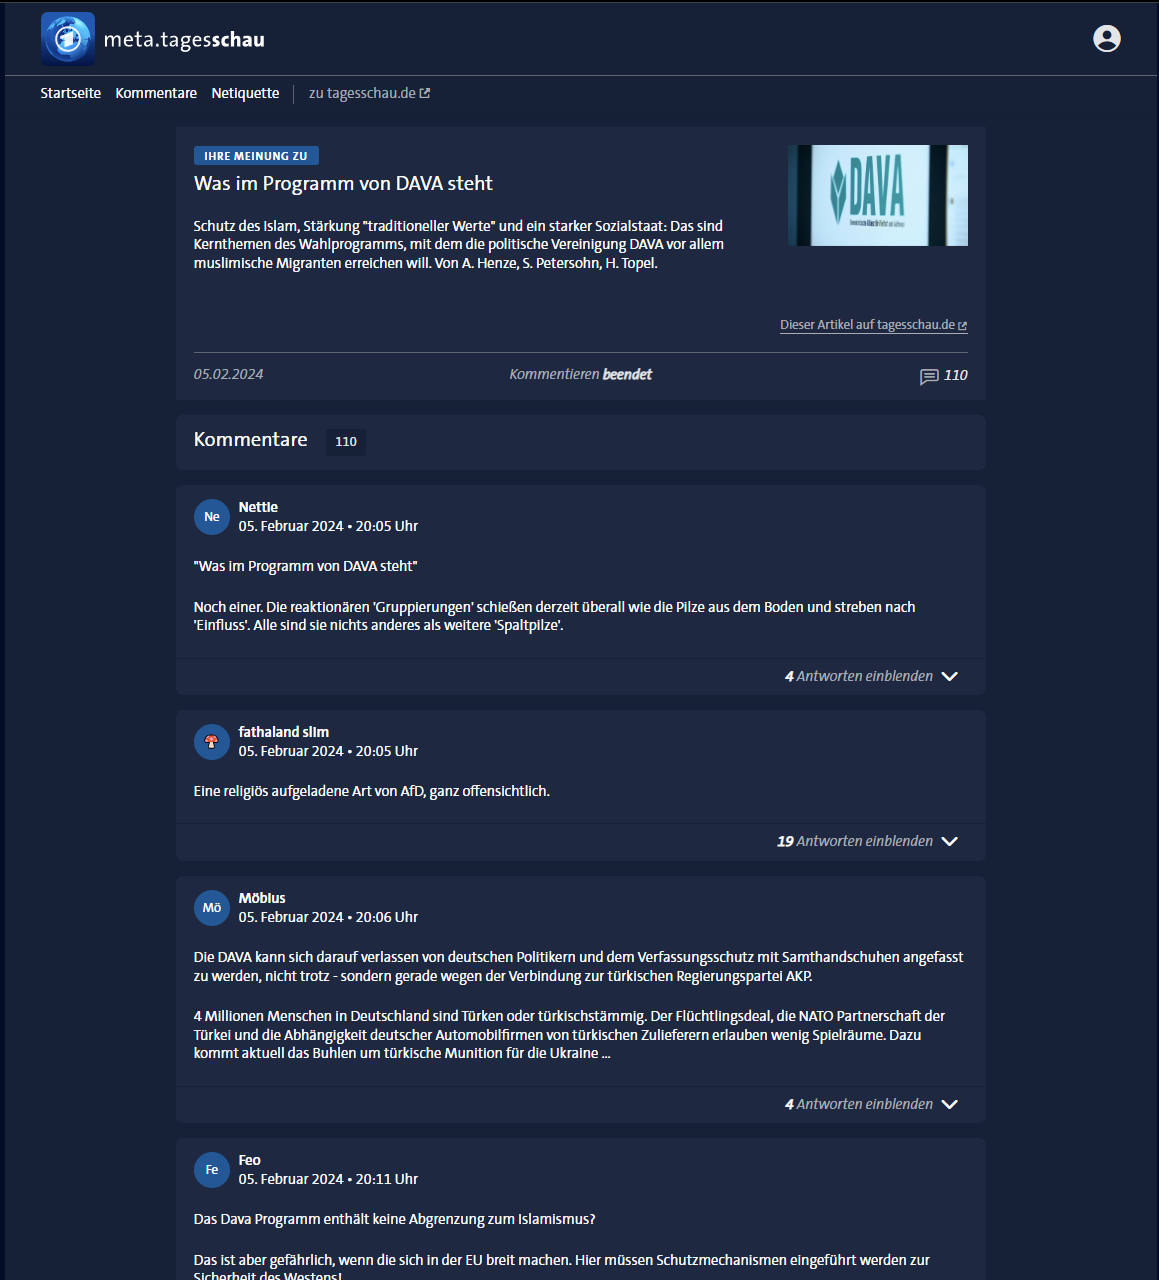
\includegraphics[width=1\linewidth]{abbildungen/Screenshot Comment Tagesschau.PNG}
    \caption{Tagesschau Kommentarsektion} 
    \label{fig:Tagesschau Kommentarsektion}
    Quelle: \fullcite{Norddeutscher_Rundfunk.2024}
\end{figure}

Aus Dieser lassen sich verschiedene Informationen beziehen.
\begin{itemize}
    \item Username
    \item Profilbild
    \item Datum und Uhrzeit des Kommentars
    \item Kommentar Text
    \item Anzahl der Antworten
    \item Anzahl der gesamten Kommentare zum Artikel
\end{itemize}

Die Kommentare werden in Seiten strukturiert und entsprechend nur teilweise zurückgegeben (engl. Paging). Dabei wird die Reihenfolge chronologisch bestimmt, beginnend mit den ersten Kommentaren. Das Konzept plant das Beziehen der ersten Seite der Kommentare.

\newpage

\begin{figure}
    \centering
    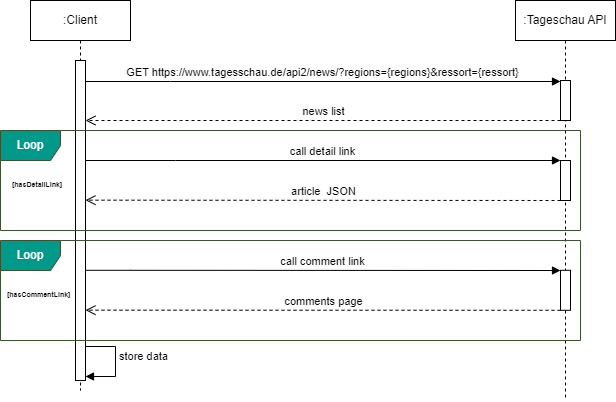
\includegraphics[width=1\linewidth]{abbildungen/Request Sequence.drawio.png}
    \caption{Abfragesequenz Datensammlung}
    \label{fig:Abfragesequenz Datensammlung}
\end{figure}
Der Ablauf der Datensammlung muss zwangsläufig mit dem initialen Abfragen der Tagesschau API starten, wie in der OpenAPI Spezifikation beschrieben. Anschließend können die Abfragen für den Artikeltext, sowie den Kommentaren stattfinden (siehe Abbildung \ref{fig:Abfragesequenz Datensammlung}). Um die Limitierung der Schnittstelle nicht zu überschreiten ist es notwendig, die zu machenden Aufrufe bestimmen zu können. Die Anzahl der benötigten Aufrufe lässt sich, auf Basis der geplanten Kommunikationsstruktur mit folgender Formel ausdrücken:

\(TotalRequests=1+(AmountArticles×2)\)

\newpage
\begin{figure}
    \centering
    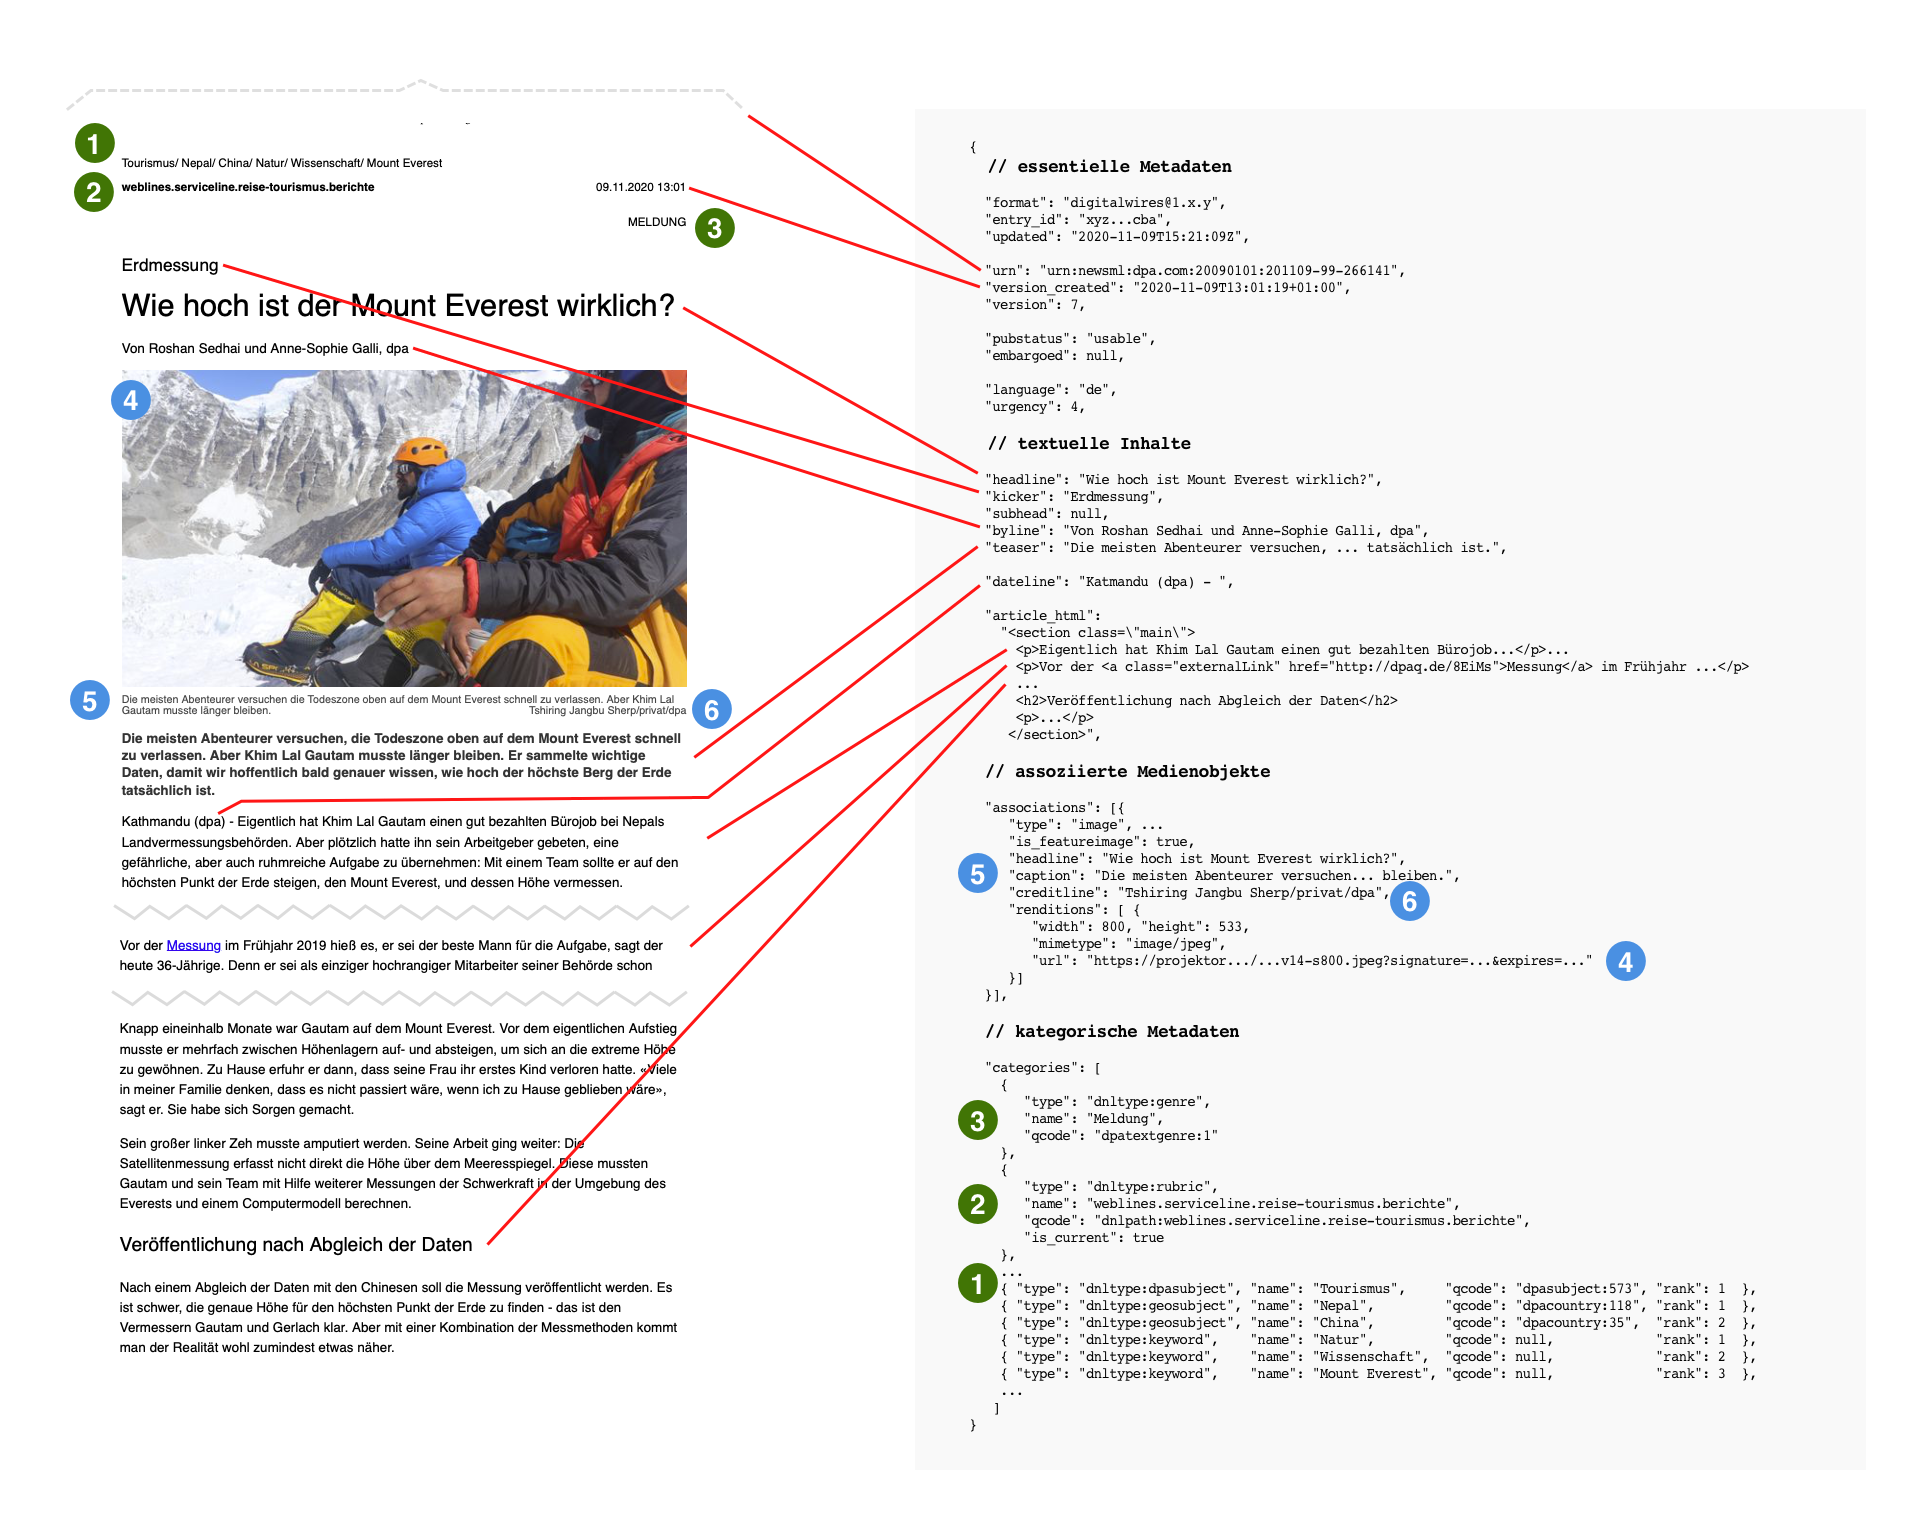
\includegraphics[width=1\linewidth]{abbildungen/dpa doc structure.png}
    \caption{Format dpa Schnittstelle}
    \label{fig:Format dpa Schnittstelle}
    Quelle: \fullcite{DpaApiDocumentation.APIs.2024}
\end{figure}
Als zweite Datenquelle wird die Deutsche Presse Agentur (dpa) angebunden. 
Diese stellt ebenfalls eine API zum konsumieren der Nachrichten bereit, jedoch ist das Angebot wesentlich weitreichender. Grundsätzlich werden drei Formen von Schnittstellen bereitgestellt:

\textbf{s3push-API}
Stellt die Daten im JSON Format über eine event-basierte Kommunikation bereit. Die Implementierung sieht eine direkte Anbindung eines S3 Buckets auf der Seite des Konsumenten vor und ermöglicht so das transportieren von neuen oder aktualisierten Topicles. Durch diesen Ansatz ist die Kommunikation zu der Schnittstelle wenig komplex und effizient, da als Konsument keine Logik zum aktualisieren der Bestandsdaten notwendig ist.\footcite[Vgl.][]{DpaApiDocumentation.APIs.2024}

\textbf{wireQ-API}
Stellt die Daten ebenfalls im JSON Format bereit, jedoch ausgegeben in einer cloud-basierten Warteschlange. Dadurch ist die Implementierung nicht an einem S3 Bucket gebunden, wodurch eine individuelle Kommunikationslogik auf Konsumentenseite notwendig ist. Erhalten bleibt dabei auch der Vorteil der Effizienz, da nur neue oder aktualisierte Daten transportiert werden.\footcite[Vgl.][]{DpaApiDocumentation.APIs.2024}

\textbf{jsonfeed-API}
Stellt die Daten ebenfalls im JSON Format technisch dar, welches strukturell jedoch Atom-XML bzw. RSS Feeds ähnelt. Beim Anfragen der Daten wird ein Vollbezug der verfügbaren Daten gestartet, welcher auch bereits abgefragte Nachrichten enthält. Entsprechend muss auf Konsumentenseite eine entsprechende Geschäftslogik implementiert werden. \footcite[Vgl.][]{DpaApiDocumentation.APIs.2024}

Für den Aufbau einer ersten Iteration der Datensammlungsumgebung ist die Anbindung an die \textit{jsonfeed-API} sinnvoll, da die Anbindung alleinstehend zunächst wenig Komplexität aufweist. 



\newpage
\subsection{Architektur und Design der Datensammlungsumgebung}

Um das Limit der Tagesschau API von 40 Anfragen pro Stunde nicht zu überschreiten, wurde folgender Batch Job konzipiert. 

\begin{figure}
    \centering
    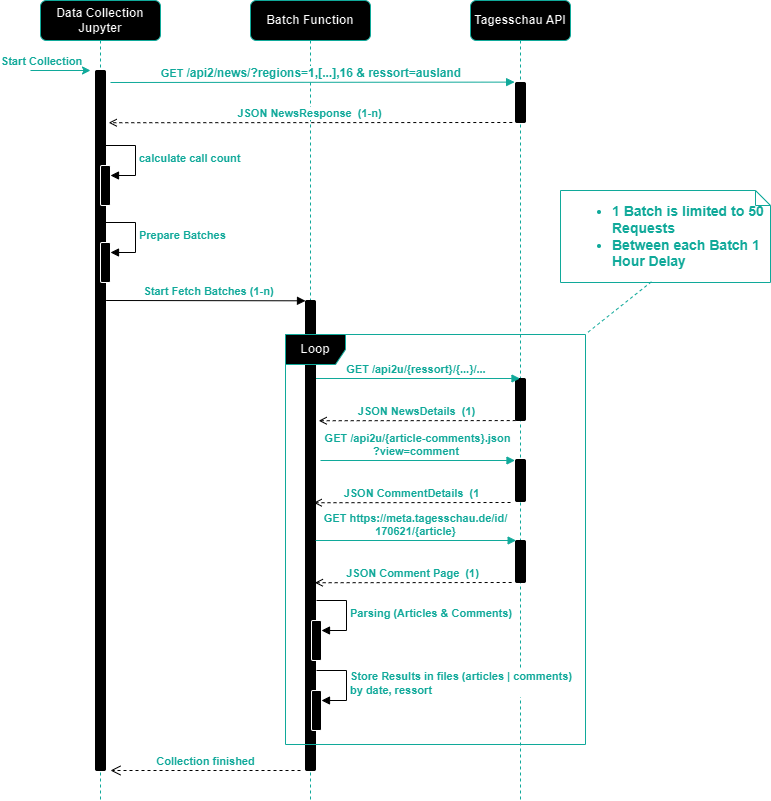
\includegraphics[width=1\linewidth]{abbildungen/image.png}
    \caption{Sequenzdiagramm Abfrage von Tagesschau Daten}
    \label{fig:Sequenzdiagramm Abfrage von Tagesschau Daten}
\end{figure}
\newpage
\section{Ergebnisse}

\subsection{Asynchrone Batch Verarbeitung von limitierten REST-APIs}
TBD

\newpage

\subsection{Explorative Analyse der Datengrundlage}
Tbd
\newpage

\subsection{Sentiment Analyse zum Validieren des Datenkorpus}
Tbd

\section{Fazit}

Analyse und Bewertung der Datensammlungsumgebung

Ausblick


%-----------------------------------
% Apendix / Anhang
%-----------------------------------
\newpage
\section*{\AppendixName} %Überschrift "Anhang", ohne Nummerierung
\addcontentsline{toc}{section}{\AppendixName} %Den Anhang ohne Nummer zum Inhaltsverzeichnis hinzufügen

\begin{appendices}
% Nachfolgende Änderungen erfolgten aufgrund von Issue 163
\makeatletter
\renewcommand\@seccntformat[1]{\csname the#1\endcsname:\quad}
\makeatother
\addtocontents{toc}{\protect\setcounter{tocdepth}{0}} %
	\renewcommand{\thesection}{\AppendixName\ \arabic{section}}
	\renewcommand\thesubsection{\AppendixName\ \arabic{section}.\arabic{subsection}}
	\section{Anhang}\label{Anhang}
Dieser Abschnitt dient nur dazu zu demonstrieren, wie ein Anhang aufgebaut seien kann.
\subsection{Quellcode}

\section{Bilder}
Auch mit Bildern.
Diese tauchen nicht im Abbildungsverzeichnis auf.

\end{appendices}
\addtocontents{toc}{\protect\setcounter{tocdepth}{2}}

%-----------------------------------
% Literaturverzeichnis
%-----------------------------------
\newpage

% Die folgende Zeile trägt ALLE Werke aus literatur.bib in das
% Literaturverzeichnis ein, egal ob sie zietiert wurden oder nicht.
% Der Befehl ist also nur zum Test der Skripte sinnvoll und muss bei echten
% Arbeiten entfernt werden.
%\nocite{*}

%\addcontentsline{toc}{section}{Literatur}

% Die folgenden beiden Befehle würden ab dem Literaturverzeichnis wieder eine
% römische Seitennummerierung nutzen.
% Das ist nach dem Leitfaden nicht zu tun. Dort steht nur dass 'sämtliche
% Verzeichnisse VOR dem Textteil' römisch zu nummerieren sind. (vgl. S. 3)
%\pagenumbering{Roman} %Zähler wieder römisch ausgeben
%\setcounter{page}{4}  %Zähler manuell hochsetzen

% Ausgabe des Literaturverzeichnisses

% Keine Trennung der Werke im Literaturverzeichnis nach ihrer Art
% (Online/nicht-Online)
%\begin{RaggedRight}
%\printbibliography
%\end{RaggedRight}

% Alternative Darstellung, die laut Leitfaden genutzt werden sollte.
% Dazu die Zeilen auskommentieren und folgenden code verwenden:

% Literaturverzeichnis getrennt nach Nicht-Online-Werken und Online-Werken
% (Internetquellen).
% Die Option nottype=online nimmt alles, was kein Online-Werk ist.
% Die Option heading=bibintoc sorgt dafür, dass das Literaturverzeichnis im
% Inhaltsverzeichnis steht.
% Es ist übrigens auch möglich mehrere type- bzw. nottype-Optionen anzugeben, um
% noch weitere Arten von Zusammenfassungen eines Literaturverzeichnisse zu
% erzeugen.
% Beispiel: [type=book,type=article]
\printbibliography[nottype=online,heading=bibintoc,title={\langde{Literaturverzeichnis}\langen{Bibliography}}]

% neue Seite für Internetquellen-Verzeichnis
\newpage

% Laut Leitfaden 2018, S. 14, Fussnote 44 stehen die Internetquellen NICHT im
% Inhaltsverzeichnis, sondern gehören zum Literaturverzeichnis.
% Die Option heading=bibintoc würde die Internetquelle als eigenen Eintrag im
% Inhaltsverzeicnis anzeigen.
%\printbibliography[type=online,heading=bibintoc,title={\headingNameInternetSources}]
\printbibliography[type=online,heading=subbibliography,title={\headingNameInternetSources}]

\newpage
\pagenumbering{gobble} % Keine Seitenzahlen mehr

%-----------------------------------
% Ehrenwörtliche Erklärung
%-----------------------------------
\section*{%
	\langde{Ehrenwörtliche Erklärung}
	\langen{Declaration in lieu of oath}}
\langde{Hiermit versichere ich, dass die vorliegende Arbeit von mir selbstständig und ohne unerlaubte Hilfe angefertigt worden ist, insbesondere dass ich alle Stellen, die wörtlich oder annähernd wörtlich aus Veröffentlichungen entnommen sind, durch Zitate als solche gekennzeichnet habe. Ich versichere auch, dass die von mir eingereichte schriftliche Version mit der digitalen Version übereinstimmt. Weiterhin erkläre ich, dass die Arbeit in gleicher oder ähnlicher Form noch keiner Prüfungsbehörde/Prüfungsstelle vorgelegen hat. Ich erkläre mich damit \textcolor{red}{einverstanden/nicht einverstanden}, dass die Arbeit der Öffentlichkeit zugänglich gemacht wird. Ich erkläre mich damit einverstanden, dass die Digitalversion dieser Arbeit zwecks Plagiatsprüfung auf die Server externer Anbieter hochgeladen werden darf. Die Plagiatsprüfung stellt keine Zurverfügungstellung für die Öffentlichkeit dar.}
\langen{I hereby declare that I produced the submitted paper with no assistance from any other party and without the use of any unauthorized aids and, in particular, that I have marked as quotations all passages which are reproduced verbatim or near-verbatim from publications. Also, I declare that the submitted print version of this thesis is identical with its digital version. Further, I declare that this thesis has never been submitted before to any examination board in either its present form or in any other similar version. I herewith \textcolor{red}{agree/disagree} that this thesis may be published. I herewith consent that this thesis may be uploaded to the server of external contractors for the purpose of submitting it to the contractors’ plagiarism detection systems. Uploading this thesis for the purpose of submitting it to plagiarism detection systems is not a form of publication.}


\par\medskip
\par\medskip

\vspace{5cm}

\begin{table}[H]
	\centering
	\begin{tabular*}{\textwidth}{c @{\extracolsep{\fill}} ccccc}
		\myOrt, \the\day.\the\month.\the\year
		&
		% Hinterlege deine eingescannte Unterschrift im Verzeichnis /abbildungen und nenne sie unterschrift.png
		% Bilder mit transparentem Hintergrund können teils zu Problemen führen
		
\includegraphics[width=0.35\textwidth]{unterschrift}\vspace*{-0.35cm}
		\\
		\rule[0.5ex]{12em}{0.55pt} & \rule[0.5ex]{12em}{0.55pt} \\
		\langde{(Ort, Datum)}\langen{(Location, Date)} & \langde{(Eigenhändige Unterschrift)}\langen{(handwritten signature)}
		\\
	\end{tabular*} \\
\end{table}

\end{document}
